\documentclass[11pt]{book}
\usepackage{qtree}
\usepackage{graphicx}
%Gummi|065|=)
\title{\textbf{Programming Languages}}
\author{Ege Emir Ozkan}
\date{}
\begin{document}

\maketitle

\chapter{Languages and Creation}

\section{Types of Programming Languages}

\subsection{Why are there so many programming languages?}

\begin{itemize}
	\item Evolution of language constructs, such as the evolution of goto based control flows to loops to nested block struuctures to object-oriantation opens new possibilities to discover.
	
	\item Special purposes, languages for scientific computing, embedding systems programming, data science.
	
	\item Subjective ideas about what is nice to use.
\end{itemize}


\subsection{What makes a language successful?}

\begin{itemize}
	\item Expressive power of the language.
	\item Ease of use for the beginners (Python)
	\item Ease of implementation, easy to write a compiler/interpreter for.
	\item Standardization (Java standard)
	\item Open source (Java, Python)
	\item Good compilers (Rust, Go)
	\item Economic backing, patronage (Swift as the offical language for Apple products, Vala for Gnome desktop.)
\end{itemize}

\subsection{Categorising Programming Languages by Syntax}

\Tree [.Languages [ .Declarative [ .Functional  Lisp Haskell ] [ .Logical Prolog ] ] [ .Imperative [ .von\ Neumann Fortran C ] [ .Scripting Python JavaScript ] [ .Object-Orianted Eiffel Java ] ] ]

\subsection{Categorising Programming Langauges by Methods of Execution}

\Tree [ .Program Assembler Compiler Interpreter  ]

\subsubsection{Assembler}

In the early days of computing, Machine Instructions were used to represent the programs, however, due to the complexity of this method, first Assemblers were produced, these assemblers assembled assembly instructions, which used one-to-one correspondence between machine instructions and their mnemonics, to machine instructions to create executable files.

\textit{Examples: x86 Assembly}


\subsubsection{Compiler}
Compilers create executables from high level languages by translating them to the Assembly or Machine Code instructions. Compilers lack the one-to-one correspondence between mnemonics and instructions that is found in assemblers, but state-of-the art compilers produce better code than any human will. Labor costs now outweigh the hardware costs.W

\textit{Examples: C, Fortran}

\subsubsection{Interpreter}
Interpreters do not produce output programs, rather, they take the input and output together and execute them together.

\textit{Examples: Python, R, Lua}

\subsubsection{Interpretation vs Compilation}
\textbf{Compilers provide} better speed through analysis and nontrival transofrmation, while \textbf{Interpreters provide} greater flexibility and through error messages better diagnostics.

\subsubsection{Virtual Machines}
By providing a target architecture that can be shared by multiple architectures called a virtual machine, source program is compiled to an intermediate representation and this representation is then interpretered through the virtual machine.

\textit{Examples: C\#, Java}

\section{Compiler Systems}
\begin{figure}[h!]
	\center
	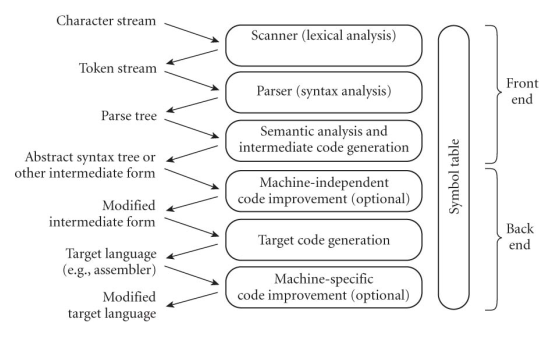
\includegraphics[scale=0.5]{../figures/01_phases_of_compilation.png}
	\caption{Model of a compiler}
\end{figure}

\subsection{Auxillary Systems}

\subsubsection{Linker}
Linker links external libraries to the program enabling usage of wider machine instructions, linker's linked library's instructions are added after the inital compilation of the source code to an incomplete set of machine instructions.
\subsubsection{Preprocessor}
Preprocessor modifies the existing source code prior to inital compilation.
\subsection{Frontend}
\subsubsection{Scanning}

Recognition of a regular language via a Definite Finite Automata to check if all of the program's tokens are well formed.

\subsubsection{Parsing}
Parsing is the checking if the source code conforms to the syntax defined by a context-free grammar.

\subsubsection{Semantic Analysis}
Semantic analysis is the checking of all the other rules not captured by the context-free grammar and the parse tree.

\chapter{Programming Language Syntax}

{\center Representation of the Context Free Grammars is the Backus-Naur Form, sometimes shortened to BNF, this representation can relaibly express any context free grammar.}

\subsection{Example}

\subsubsection{Example grammar}
\end{document}
